\chapter{附录}\label{ch:appendix}

\section{特殊内核功能的实现}\label{sec:9-special-kernel-features}

RME 可以支持诸多某些其他操作系统提供的特殊功能，诸如CPU热插拔、内存热插拔、隔离内核、准虚拟化等等。下面简述它们的实现思路。

\subsection{CPU热插拔的实现}\label{subsec:9-cpu-hotplug}

CPU热插拔分为两个功能，一个是热插，也即插入新的CPU，增加CPU的数量；另外一个是热拔，也即从插槽上拔出CPU，减少CPU的数量。RME 对该功能的支持依赖于底层硬件平台提供的硬件级别支持，并且都要用定制的内核功能调用完成。

对于热插，可以在检测到物理CPU封装插入后，初始化该处理器并且创建应有的 Init 线程，然后即可使用这些处理器核。

对于热拔则是相反的，需要停止相应处理器的活动，并且其他处理器核不应该再向该处理器发送IPI。然后，我们才能把这个物理CPU封装移除。

\subsection{内存热插拔的实现}\label{subsec:9-memory-hotplug}

内存热插拔也分为两部分，一部分是增加内存，另一部分是减少内存。RME 对该功能的支持依赖于底层硬件平台提供的硬件级别支持，并且也都要用定制的内核功能调用完成。

对于增加内存的情况，如果是增加用户态内存，只要将这些内存对应的物理页框加入到某个用户页表中即可。如果需要增加内核内存，那么需要先暂停其他处理器的运行，然后向内核页表中增加新的页面并修改内核页表以反映这一更改，最后再恢复其他处理器的运行。在完成所有操作后还要做一个TLB刷新操作。

对于减少内存的情况，如果是减少用户态内存，需要用户态库确定现在这些物理页面没有被映射。此时，可以直接除去这些页面的映射并拔出该内存条。如果是减少内核内存，那么需要首先暂停其他处理器的运行，然后将要拔出的内存上的数据拷贝到空白的物理页面上，并修改内核页表以反映这一更改，最后再恢复其他处理器的运行。在完成所有操作后也要做一个TLB刷新操作。

\subsection{隔离内核的实现}\label{subsec:9-isolated-kernel}

由于 RME 是一个微内核操作系统，因此，就像 Barrelfish 那样\hyperref[cite:9-1]{{[}1{]}}，可以很方便地在一台物理机器上运行 RME 的多个实例。每个实例可以管理一个或多个CPU核，然后在用户态通过多个操作系统共享内存或者网络实现通信即可。这种方式不要求CPU间的缓存是同步的，也不要求各个CPU含有的功能是一样的，甚至不要求各个CPU的指令集和架构是一样的。如果在此种系统中用到了多种架构的处理器，那么就需要针对它们分别移植 RME 和用户态库。

\needspace{14\baselineskip}
比如，如果存在如下图所示的SoC或单板机\footnote{HMMU指硬件填充的MMU，SMMU指软件填充的MMU}，那么是可能在全部的核上运行 RME 的，然后通过不同的子系统间共享内存来完成信息传递。

\begin{figure}[H]
    \centering
    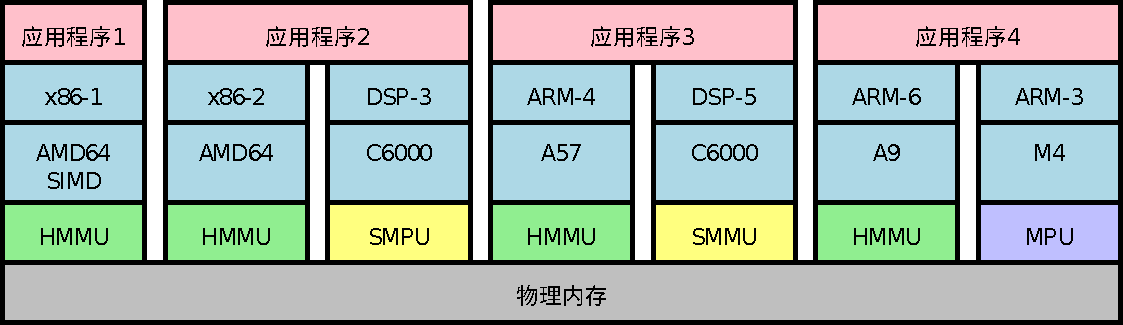
\includegraphics[width=0.72\textwidth]{Figure/image14.pdf}
    \caption{基于异构多核的隔离内核的典型实现方案}
    \label{fig:9-1-heterogeneous-multicore-isolated-kernel}
\end{figure}

\needspace{14\baselineskip}
上图所示为不同架构共同运行的一个例子。在不同的NUMA节点上各运行一个 RME 的实例也是可行的，如下图所示：

\begin{figure}[H]
    \centering
    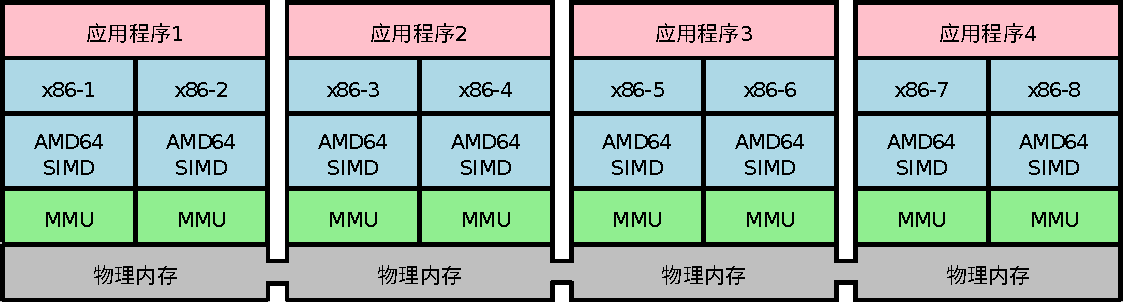
\includegraphics[width=0.72\textwidth]{Figure/image15.pdf}
    \caption{基于NUMA的隔离内核的典型实现方案}
    \label{fig:9-2-numa-isolated-kernel}
\end{figure}

\subsection{无节拍内核的实现}\label{subsec:9-tickless-kernel}

无节拍内核要求系统的每个CPU核都具备一个独立可编程的高精度定时器，并且由该高精度定时器产生可变的调度器时间中断。时间片和定时器填充值之间的比例可以由实现者按需自由决定。为了方便实现无节拍内核，系统提供两个函数\_RME\_Tim\_Future和\_RME\_Tim\_Elapse；如果不实现无节拍内核可以不必理会它们。

为了使定时器在潜在的下一超时时点产生中断，在每次当前线程的剩余时间片发生变动后\footnote{如各类中断向量的出口处}都需要将该时间设置成硬件定时器的下一次超时时间。有三种情况可能导致剩余时间片发生变动：（1）由任意原因引起的上下文切换\footnote{也存在上下文切换前后线程的剩余时间片刚好相同的巧合；此时并不需要重编程定时器}，（2）在系统调用向量中使用RME\_SVC\_THD\_TIME\_XFER且当前线程的时间片因此发生改变，（3）发生了定时器中断\footnote{发生这个中断不一定意味着某线程耗尽了自己的时间片，也可能意味着硬件定时器的最长可配置超时时间不够长而需要将一个定时分多段完成}。在某些架构上，重编程定时器耗时可能较久，而发生中断未必一定引起剩余时间片的变动，因此可以自行查询判断进入中断前后的当前线程时间片变动来决定是否需要重编程定时器；定时器中断是一个特例，它肯定需要一次定时器重编程，因而可免去此查询。

内核提供了函数\_RME\_Tim\_Future用于得到该超时时间。如果这段时间的长度超过了硬件定时器能支持的范围，只要将硬件定时器的超时时间设置成允许的最大值即可；RME的设计保证只有实际经过的时间才会从线程剩余时间中抵扣掉，因此不用担心线程剩余时间丢失。

\begin{xltabular}{\textwidth}{@{}>{\hsize=0.5279\hsize\raggedright\arraybackslash}X>{\hsize=1.4721\hsize\raggedright\arraybackslash}X@{}}
\caption{得到最近超时时间片数}\label{tab:9-1-latest-timeout-slices}\\
\toprule
函数原型 & rme\_ptr\_t \_RME\_Tim\_Future(void)\tabularnewline
\endfirsthead
\toprule
函数原型 & rme\_ptr\_t \_RME\_Tim\_Future(void)\tabularnewline
\midrule
\endhead
\bottomrule
\endlastfoot
意义 &
得到距离未来最近一次超时的时间片数，可根据此设置系统定时器的下一次超时时间。\tabularnewline
返回值\strut
 & rme\_ptr\_t

距离未来最近一次超时的时间片数。\strut
\tabularnewline
参数 & 无。\tabularnewline
\end{xltabular}

为了使所有线程消耗的时间都能得到精准的记录，需要在所有可能上下文切换或修改时间片\footnote{除了定时器中断（它会调用\_RME\_Tim\_Handler）以外的各中断向量入口处；严格地讲，如果能够判断本次中断不发生线程切换，也不通过RME\_SVC\_THD\_TIME\_XFER修改当前线程的时间片，则无需调用\_RME\_Tim\_Elapse，但判断线程切换是否发生很困难，且\_RME\_Tim\_Elapse开销很低，因此推荐在所有中断向量的入口处都调用它}的时点前从当前线程中抵扣已消耗的时间。内核为此提供了函数\_RME\_Tim\_Elapse用于记录消耗的时间。

\begin{xltabular}{\textwidth}{@{}>{\hsize=0.5279\hsize\raggedright\arraybackslash}X>{\hsize=1.4721\hsize\raggedright\arraybackslash}X@{}}
\caption{记录时间流逝数}\label{tab:9-2-record-elapsed-time}\\
\toprule
函数原型 & void \_RME\_Tim\_Elapse(rme\_ptr\_t Slice)\tabularnewline
\endfirsthead
\toprule
函数原型 & void \_RME\_Tim\_Elapse(rme\_ptr\_t Slice)\tabularnewline
\midrule
\endhead
\bottomrule
\endlastfoot
意义 &
在发起潜在的上下文切换前记录当前线程已使用的时间片数。\tabularnewline
返回值 & 无。\tabularnewline
参数\strut
 & rme\_ptr\_t Slice

距离上次调用\_RME\_Tim\_Elapse或\_RME\_Tim\_Handler以来经历的时间片数。\strut
\tabularnewline
\end{xltabular}

值得注意的是，虽然无节拍内核的CPU功耗更低，但其实时性未必更好，因为它势必包含在上下文切换前的时间流逝登记，以及在上下文切换后对定时器的重编程。这都可能增加上下文切换临界区的长度，并对系统的实时性产生负面影响。而且，内核向定时器端点发送的信号也将失去周期性，用户态不再能够依赖于它。

在使用无节拍内核时，必须将RME\_TIMESTAMP宏定义为对某个独立的单向自增计数器\footnote{这种计数器通常可以在CPU性能监控单元（Performance Monitoring
  Unit，PMU）或全局计时器中找到；部分架构如x86等也提供专用的、恒常递增（CONSTANT\_TSC）和永不停息（NONSTOP\_TSC）的RDTSC指令}的读取，这可以使时间戳在任何时候都是全局的最新值，从而保证权能操作安定期的安全性。

\subsection{处理器休眠的实现}\label{subsec:9-processor-sleep}

处理器休眠臭名昭著地难以正确实现；漫不经心的设计轻则导致唤醒丢失、系统卡顿，重则导致永久休眠、机器死机。处理器对休眠指令的定义可以分为``瞻前顾后型''、``仅顾后型''和``仅触发型''，三种定义在实现策略上区别很大。如果担心无法正确实现休眠，则可以将其略去。系统的功耗会稍高，这是不休眠的唯一代价。

\subsubsection{``瞻前顾后''型}\label{subsubsec:9-sleep-look-before-and-after}

这是硬件设计最复杂、软件使用最简单的休眠指令定义\footnote{如 ARMv7-M 的设置 SEVONPEND 后的 WFE 指令}。此种休眠指令不论处理器总中断使能与否，行为都完全一致。它（1）在执行前总会原子性地检查是否有中断已经悬起，如果是则将自己当作 NOP 执行，不进入休眠，而（2）在执行后则总会检查当前是否有新的中断悬起或触发，如果是则立刻退出休眠，恢复指令执行。

对于此类型，只需要在休眠时简单地执行休眠指令即可，无需担心中断唤醒丢失。

\subsubsection{``仅顾后''型}\label{subsubsec:9-sleep-after-only}

这是硬件设计和软件使用都较复杂的休眠指令定义\footnote{如某些不标准的 RISC-V 处理器的 WFI 指令；标准的 WFI 指令是``瞻前顾后''型}。此种休眠指令不论处理器总中断使能与否，行为都完全一致。但与``瞻前顾后''型不同，它在执行前不检查是否有中断已经悬起，而是仅在执行后检查当前是否有新的中断悬起或触发，如果是则立刻退出休眠，恢复指令执行。

对于此类型，在关中断下执行则需要警惕中断唤醒丢失问题。如果不做特别处理，而在关闭中断后到在执行休眠指令前有新的中断悬起，这些悬起的中断唤醒就可能会丢失。一个幼稚的做法是，先判别是否有悬起的中断，如果没有再进入休眠：如果判断时没有中断悬起，但新的中断在判断结束后、休眠执行前悬起，该新到中断唤醒一样会丢失。

如果不在乎中断丢失，则只需要在休眠时简单地执行休眠指令即可。如果不能容忍中断丢失，则必须将其作为下一小节所述的``仅触发''型来处理。不过，部分处理器存在配置开关以将休眠指令的行为转换为上一小节所述的``瞻前顾后''型；如果能找到这样的开关，也可以直接打开它。

\subsubsection{``仅触发''型}\label{subsubsec:9-sleep-trigger-only}

这是硬件设计最简单，但软件使用最复杂的休眠指令定义\footnote{如 x86 的 HALT 指令}。此种休眠指令只能在处理器总中断开启时使用，且它一旦使用处理器就立即停止并等待新的中断来临。如果在关中断时误执行了此类指令，则处理器会因为无法接受中断而直接锁死，导致机器永久死机。这给 RME 造成了麻烦：RME 总是在系统调用中断上下文------此时中断必然关闭------中执行休眠指令，因为休眠功能是通过内核功能调用提供的。而 Linux 等宏内核则不存在此问题，因为它们有真正的、开启中断的内核空闲线程来负责休眠。

对于此类型，我们需要伪造一个类似于 Linux``内核线程''的环境来调用休眠指令。具体地：

（1）编写一段代码作为``内核线程''，在其中循环调用休眠指令。它不需要含有任何其它内容，也不需要一个独立的栈。

（2）一旦在 \_RME\_Svc\_Handler 中检测到休眠请求，就用汇编退出中断上下文到该``内核线程''\footnote{而非通常的返回用户态}，且退出到该``内核线程''时要同步开启中断。为此可以现场伪造一个返回栈；该``内核线程''的栈仍使用当前内核栈，同时保存当前内核上下文到当前内核栈上。

（3）当休眠后的首个中断来临时，检测中断打断的是否是``内核线程''。如果是，记录该中断已发生，但暂不运行它的中断向量而是恢复内核上下文，继续完成 \_RME\_Svc\_Handler 的执行。``内核线程''运行结束与否无需关心。

（4）在 \_RME\_Svc\_Handler 运行结束后扫描中断发生记录，运行被推迟的中断向量。最后按照通常的方式返回用户态。

这样一来，休眠指令就在开启中断的前提下被调用，不会导致睡死，而处理器被唤醒后会继续执行之前的内核功能调用，直到该调用处理完毕才会继续处理中断向量，不会在单处理器上导致内核重入。

\subsection{协处理器上下文的保存和恢复}\label{subsec:9-coprocessor-context-switch}

协处理器指浮点处理器、向量处理器等CPU扩展模块，它们也有自己的上下文；无论是否有多个线程共享同一个协处理器，其上下文都必须小心处理，不然除了会造成程序错乱，还会导致协处理器寄存器组变成一个巨大的隐蔽存储通道。这和只关心时间隔离而不关心空间隔离的 RMP 非常不同。此外，RME 中还有一类寄存器状态不受信任的准虚拟化专用线程，这类线程的协处理器需要更加小心处理，因为它报告的协处理器状态也是不受信任的。

掌管协处理器上下文切换的主要函数是\ref{subsubsec:7-coprocessor-register-set-functions}
中介绍的 \_\_RME\_Thd\_Cop\_Swap，它负责在线程上下文切换时一并保存和恢复该协处理器的上下文。协处理器的保存和恢复在它中实现。

根据处理器硬件层面对协处理器控制提供的功能模型，协处理器可以分为``常开型''、``关-开型''、``关-初-用型''和``关-初-净-脏型''，其中每一种都在前一种的基础上提供了更多控制功能以优化其上下文切换性能，其最优切换策略也愈发复杂。当然，每一种类型都可以以性能为代价使用它之前的类型的切换策略；当（1）对信息安全要求非常高、（2）拿不准切换策略应当如何实现、（3）怀疑当前策略实现有误时，可以一律使用``常开''型的切换策略。

\subsubsection{``常开''型}\label{subsubsec:9-coproc-always-on}

这是最简单的协处理器控制模型。在这种模型下，如果硬件层面实现了该协处理器，则它将在硬件上电时永远开启，且不可能关掉，或者软件环境大多默认开启\footnote{如 x86 的 MMX 协处理器；虽然它有开关，但基本属于标配，可以作为``常开''型处理}。此类协处理器只是名义上的协处理器，它甚至可以作为通用寄存器组的一部分进行处理，因此其切换策略是不言自明的：在任何时候都切换该协处理器寄存器组。当然，系统中的一切线程的上下文属性 Attr 都必须含有该协处理器。

在该策略下无需对准虚拟化专用线程进行任何特殊处理。

\subsubsection{``关-开''型}\label{subsubsec:9-coproc-on-off}

这是次简单的协处理器控制模型。在这种模型下，硬件实现了一个在系统启动时默认关闭的协处理器，必须打开该其开关才能使用，否则会产生异常\footnote{如 MIPS 的 COP1 浮点协处理器，它提供一个简单的开关控制位}。此时，可按如下策略切换该协处理器上下文：

首先（1）判断当前线程的上下文属性 Attr\_Cur 是否包括该协处理器；如果包括，则将该协处理器打开并将其上下文保存到当前线程上下文结构体中，如果不包括则什么都不做。然后（2）判断新线程的上下文属性 Attr\_New 是否包括该协处理器；如果包括，则将该协处理器打开并从新线程上下文结构体中恢复上下文到协处理器中，如果不包括则关闭该协处理器。

在该策略下无需对准虚拟化专用线程进行任何特殊处理，除非协处理器的开关状态也由它控制的寄存器报告。由于它报告的协处理器开关状态并不可信，协处理器的最终开关状态应和上下文属性强制保持一致。这一点也适用于后续类型，在下文中不再赘述。

不建议在此类硬件下使用``切换后关闭''-``异常''-``开启''循环策略\footnote{相当多数操作系统采取这种策略}来实现协处理器状态的软件懒保存，因为这种策略会恶化最坏执行时间：首先，所有架构的协处理器都存在大小不等的开关开销，而此策略会增加开关次数；其次，如果两个交替切换的线程都频繁使用协处理器，则每次线程切换都产生一次额外的协处理器开启异常。事实上协处理器状态的保存可以拖到最后一刻------比如新线程要开始使用协处理器之前，或者当前线程的协处理器状态结构体必须更新之前\footnote{那些查询寄存器的内核功能调用可能会读取协处理器状态}------才去做，但这需要记录当前协处理器状态的所属线程并时刻跟踪之，会造成额外的移植者心智负担。只有在平均性能远比最坏执行时间重要时才可以这样做，且在这样做时对处理器微架构的猜测执行（Speculative
execution）机制必须有清晰了解，否则可能引起协处理器状态泄露\footnote{为避免这种情况，官方移植永远不会带着一个线程的协处理器上下文去执行另一个线程，即使协处理器是关闭的}。

不过，使用``初始关闭''-``初次异常''-``永久常开''策略将此类硬件转化为``关-初-脏''型并采取其``切换策略一''则是值得鼓励的，因为异常仅会在线程初次使用协处理器时引发一次。

\subsubsection{``关-初-脏''型}\label{subsubsec:9-coproc-off-initial-dirty}

这是较常见的协处理器控制模型。在这种模型下，硬件不仅实现了协处理器开关，还会实时探测协处理器是否被使用过。如果协处理器未被开启，则使用该协处理器会产生异常；如果协处理器被开启但未被实际访问过，则``脏''位不会被硬件置位，直到该协处理器被第一次实际访问\footnote{如 ARMv7-M 的 FPv4 和 FPv5 浮点处理器}。此时，针对该协处理器的上下文有两种处理策略：

第一种策略将``脏''位当作``初始状态''的象征。它是最常使用的策略，有利于跳过在上下文属性中声明协处理器但从未碰过它\footnote{即便线程的整个生命周期都不使用协处理器也要声明使用，这有利于提高前向兼容性}的线程的不必要的上下文保存和恢复，是 RME 的官方移植中使用的策略；该策略类似于 RMP 采取的策略。该策略的具体操作如下表所示。

\begin{xltabular}{\textwidth}{@{}>{\hsize=0.9261\hsize\raggedright\arraybackslash}X>{\hsize=0.6708\hsize\raggedright\arraybackslash}X>{\hsize=1.4031\hsize\raggedright\arraybackslash}X@{}}
\caption{``关-初-脏''型切换策略一}\label{tab:9-3-off-initial-dirty-strategy-1}\\
\toprule
当前线程 & 新线程 & 操作\tabularnewline
\endfirsthead
\toprule
当前线程 & 新线程 & 操作\tabularnewline
\midrule
\endhead
\bottomrule
\endlastfoot
\multirow{3}{=}{\makecell[l]{不包括协处理器\\（不在Attr中）}} & 不包括协处理器\strut
 & 什么也不需要做\strut
\tabularnewline
& 协处理器没动过 & 开启协处理器\tabularnewline
& 协处理器使用过 &
开启协处理器并从新线程上下文结构体中恢复协处理器上下文\tabularnewline
\multirow{3}{=}{\makecell[l]{协处理器没动过\\（初始）}} & 不包括协处理器\strut
 & 关闭协处理器\strut
\tabularnewline
& 协处理器没动过 & 什么也不需要做\tabularnewline
& 协处理器使用过 &
从新线程上下文结构体中恢复协处理器上下文\tabularnewline
\multirow{3}{=}{\makecell[l]{协处理器使用过\\（脏）}} & 不包括协处理器\strut
 & 先保存协处理器上下文到当前线程上下文结构体，再重新初始化协处理器上下文，最后关闭协处理器\strut
\tabularnewline
& 协处理器没动过 &
保存协处理器上下文到当前线程上下文结构体并重新初始化协处理器上下文\tabularnewline
& 协处理器使用过 &
保存协处理器上下文到当前线程上下文结构体并从新线程上下文结构体中恢复协处理器上下文\tabularnewline
\end{xltabular}

在该策略下需要特别警惕准虚拟化专用线程，因为它报告的``脏''位并不可靠。它可以在修改过协处理器上下文后在用户态清零``脏''位以报告一个伪造的``初始状态''\footnote{这种状况只有存在多核CPU时会发生，其它核可以对该数据结构并行地进行修改}，这样就可以将自己的协处理器状态泄露给新线程。因此，只要当前线程是准虚拟化专用线程，必须无视其``脏''位的状态并认为它使用过协处理器。不过，在它报告自己处于``初始状态''时，可以不必保存协处理器上下文到它的上下文结构体；这并不会伤害诚实的准虚拟化专用线程。

第二种策略将``脏''位当作``保存过上下文''的象征。它有利于跳过间歇使用协处理器的线程中不使用协处理器的执行段的不必要的上下文保存，在所有线程都实际使用协处理器时能提高平均性能，但于最坏执行时间并无益处。该策略的具体操作如下表所示。

\begin{xltabular}{\textwidth}{@{}>{\hsize=0.7814\hsize\raggedright\arraybackslash}X>{\hsize=1.0349\hsize\raggedright\arraybackslash}X>{\hsize=1.1837\hsize\raggedright\arraybackslash}X@{}}
\caption{``关-初-脏''型切换策略二}\label{tab:9-4-off-initial-dirty-strategy-2}\\
\toprule
当前线程 & 新线程 &
操作\tabularnewline
\endfirsthead
\toprule
当前线程 & 新线程 &
操作\tabularnewline
\midrule
\endhead
\bottomrule
\endlastfoot
\multirow{2}{=}{\makecell[l]{不包括协处理器\\（不在Attr中）}} & 不包括协处理器\strut
 & 什么也不需要做\strut
\tabularnewline
& 协处理器保存过 &
开启协处理器并从新线程上下文结构体中恢复协处理器上下文\tabularnewline
\multirow{2}{=}{\makecell[l]{协处理器保存过\\（干净）}} & 不包括协处理器\strut
 & 关闭协处理器（并清空协处理器上下文）\strut
\tabularnewline
& 协处理器保存过 &
从新线程上下文结构体中恢复协处理器上下文\tabularnewline
\multirow{2}{=}{\makecell[l]{协处理器未保存\\（脏）}} & 不包括协处理器\strut
 & 先保存协处理器上下文到当前线程上下文结构体，再清零当前线程的``脏''位，最后关闭协处理器（并清空协处理器上下文）\strut
\tabularnewline
& 协处理器保存过 &
先保存协处理器上下文到当前线程上下文结构体，再清零当前线程的``脏''位，最后从新线程上下文结构体中恢复协处理器上下文\tabularnewline
\end{xltabular}

在该策略下无需对准虚拟化专用线程进行任何特殊处理\footnote{在该策略下，新线程的``脏''位必定是清零的}。即便它报告的``脏''位的状态并不可信，在切换到它时协处理器上下文也总是被重新装载，不可能通过恶意操纵此位将自己的上下文泄露出去。

注：理论上讲，操作系统可以在线程上下文结构体中引入一个额外的变量来记录``初始''状态，该状态用来单独指示线程是否曾碰过协处理器，这样就可以将``关-初-脏''型转化为下一小节所述的``关-初-净-脏''型以进一步提升性能。但是，这会引入额外的复杂性和内存消耗，且引入该变量会给代码读者造成额外的心智负担，因此 RME 的官方移植不采取这种方案。

\subsubsection{``关-初-净-脏''型}\label{subsubsec:9-coproc-off-initial-clean-dirty}

这是最先进也最复杂的协处理器控制模型，它为协处理器的所有状态都提供了原生的独立指示，因此可以获得最好的性能。如果协处理器未被开启，则使用该协处理器会产生异常；如果协处理器被开启但未被实际访问过，则协处理器会停留在``初始''状态，直到该协处理器被第一次实际访问\footnote{如RISC-V的 F、D 和 Q 标准扩展}，此时硬件会使协处理器会进入``脏''状态；在线程切换的协处理器上下文保存结束后，软件并不会把``脏''状态修改为``初始''状态，而是修改为``干净''状态；在``干净''状态下的任何协处理器访问也会导致硬件把协处理器变为``脏''状态。其切换策略如下表所示：

\begin{xltabular}{\textwidth}{@{}>{\hsize=0.7464\hsize\raggedright\arraybackslash}X>{\hsize=1.0405\hsize\raggedright\arraybackslash}X>{\hsize=1.2131\hsize\raggedright\arraybackslash}X@{}}
\caption{``关-初-净-脏''型切换策略}\label{tab:9-5-off-initial-clean-dirty-strategy}\\
\toprule
当前线程 & 新线程 &
操作\tabularnewline
\endfirsthead
\toprule
当前线程 & 新线程 &
操作\tabularnewline
\midrule
\endhead
\bottomrule
\endlastfoot
\multirow{3}{=}{\makecell[l]{不包括协处理器\\（不在 Attr 中）}} & 不包括协处理器\strut
 & 什么也不需要做\strut
\tabularnewline
& 协处理器没动过 & 开启协处理器\tabularnewline
& 协处理器保存过 &
开启协处理器并从新线程上下文结构体中恢复协处理器上下文\tabularnewline
\multirow{3}{=}{\makecell[l]{协处理器没动过\\（初始）}} & 不包括协处理器\strut
 & 关闭协处理器\strut
\tabularnewline
& 协处理器没动过 & 什么也不需要做\tabularnewline
& 协处理器保存过 &
从新线程上下文结构体中恢复协处理器上下文\tabularnewline
\multirow{3}{=}{\makecell[l]{协处理器保存过\\（干净）}} & 不包括协处理器\strut
 & 重新初始化协处理器上下文并关闭协处理器\strut
\tabularnewline
& 协处理器没动过 & 重新初始化协处理器上下文\tabularnewline
& 协处理器保存过 &
从新线程上下文结构体中恢复协处理器上下文\tabularnewline
\multirow{3}{=}{\makecell[l]{协处理器未保存\\（脏）}} & 不包括协处理器\strut
 & 先保存协处理器上下文到当前线程上下文结构体，再将当前线程转变为``干净''状态，再重新初始化协处理器上下文，最后关闭协处理器\strut
\tabularnewline
& 协处理器没动过 &
先保存协处理器上下文到当前线程上下文结构体，再将当前线程转变为``干净''状态，最后重新初始化协处理器上下文\tabularnewline
& 协处理器保存过 &
先保存协处理器上下文到当前线程上下文结构体，再将当前线程转变为``干净''状态，最后从新线程上下文结构体中恢复协处理器上下文\tabularnewline
\end{xltabular}

在该策略下需要特别警惕准虚拟化专用线程，因为它报告的任何协处理器状态都不可靠\footnote{在该策略下，新线程不可能处于``脏''状态}。它可以在修改过协处理器上下文后在用户态修改协处理器状态寄存器以报告一个伪造的``初始''状态，这样就可以将自己的协处理器状态泄露给新线程。因此，只要当前线程是准虚拟化专用线程，必须将其报告的``初始''状态当作``干净''状态来处理。

\subsection{用户态页表直管的实现}\label{subsec:9-user-mode-page-table-management}

虽然 RME 的内核极尽所能地提供了对页表的高效抽象，但出于最坏执行时间可控、用户态灵活性最大化等考虑，RME 的每级页目录都对应于一个权能，页表操作粒度细但效率低。一方面，在一般无需修改页表映射的微控制器场合\footnote{内存保护单元的页表纯粹是软件模拟的，如果不需要修改映射则完全不需要它们}，大量的页目录及其权能会消耗本就不多的系统内存；另一方面，在需要频繁或大量修改页表的微处理器场合\footnote{这一般是出于缺页中断，而缺页中断是实现懒请求的底层手段；在那些在乎平均性能和资源利用率的操作系统（如云计算等）中，懒请求又是一系列效率优化的基础支撑}，页表操作的低效率会拖累整个系统的吞吐率和尾延迟。考虑到不同场景下对内存管理的需求大相径庭，RME 认为内存管理的权责在本质上归于用户\footnote{所有的性能问题在本质上都是权责问题}：用户有责任在需求特殊时自行实现页表管理。

将 RME\_PGT\_RAW\_ENABLE 定义为1即开启用户态页表直管功能。该功能一旦启用，页表的管理即由用户态的可信进程全权控制，该可信进程本质上是内核的一部分\footnote{攻破它和攻破内核的后果完全是一样的，换言之，它属于可信计算基（Trusted
  Computing Base，TCB）}，和内核的区别仅仅在于（1）它表面上运行在用户态，（2）由于前款原因，它可以被抢占，因此不影响系统的最坏执行时间。此时，页表相关的系统调用和底层相关函数会发生一些变化；有关这些变化可参见\ref{subsec:7-general-macro-definitions}
，在此不再赘述。接下来将分两小节阐述极端场景下的用户态页表直管设计。

\subsubsection{深度嵌入式场景}\label{subsubsec:9-deep-embedded-scenario}

深度嵌入式场景中最常用的是微控制器（MCU），其系统的特点是专机专用、实时可靠、预算不多、资源吃紧，其进程一经建立就基本不修改其地址空间映射。此时，除非要实现动态页功能\footnote{部分 RISC-V 微控制器出于成本考虑采用了简化的微架构，不能生成精确的访存越权异常，因而无法使用动态页功能；此时，基本没有不开启用户态页表直管的理由}，保留页目录数据结构及其权能的意义十分有限。

在深度嵌入式场景中，推荐的做法是在工程编译时就生成能够直接填充给内存保护单元（MPU）的表格，并在系统初始化时直接用这些表格初始化MPU以彻底省去内核页表开销；这些表格都是常量，因此可以放在ROM中以进一步削减内存用量。此外，这种方法还可以针对MPU的特性生成配置数据，能比路径压缩页表更好地适配基址-长度型MPU。与 RME 配套的 RVM 虚拟机监视器提供了这一功能；有关如何开启这一功能，请参见 RVM 的手册。

\subsubsection{云原生服务场景}\label{subsubsec:9-cloud-native-scenario}

与深度嵌入式场景相比，云原生服务场景是另一个极端，在其中唱主角的是基于微处理器的标准机架式服务器。它们往往拥有TB量级的内存，因此页表所占的内存空间不值一提。然而，（1）微处理器系统的动态性非常高，进程的创建与销毁、内存的分配与释放十分频繁，由此所致的页表操作都是大开大合的，有时甚至会一次性映射或撤销几十万乃至上百万个页面。如果每次页面映射或撤销都要操作一次页表权能，造成的性能开销将不可忽视。而且，（2）页目录在创建时需要内核将其清零，这会大大拖慢内核的最坏执行时间，如果连续创建多个页目录可能会引入密集的抖动，从而引起尾延迟超标\footnote{在客户端往往表现为程序卡顿、鼠标不跟手，在服务端往往表现为响应波动大、服务质量差}。此外，（3）缺页中断也会引入巨量的页表操作；即便在那些不使用页面交换算法的内存充足的系统上，缺页中断在推迟数据拷贝、按需同步数据方面也有巨大的作用\footnote{如 Linux 的 fork 调用会尽力推迟内存拷贝直到相应的页真的被修改；类似的机制在 mmap 中也存在}，因此对其进行迅捷响应仍十分必要。最后，（4）服务器系统要分配多少内核专用内存难以决定，因此其内核对象登记表 Kotbl 总是覆盖整个内存范围；此时，内核内存与用户内存的动态划界以及内核对象的管理本就需要一个用户态可信进程来包办，再在其中追加一个页表管理功能就再自然不过了。

云原生服务场景中的推荐做法并无一定之规，但总的原则是（1）减少同等页表操作工作量下的IPC的次数，（2）将页表和其它内存对象整合成便于使用的粗粒度实体提供给应用程序，（3）在存在多个管理层次时尽量避免层层加码，以及（4）在设计机制时充分考虑到进程间的时空隔离。当然，如果不频繁操作地址空间或无苛刻的性能要求，不使用用户态页表直管也无甚不妥。

\section{内存保护单元的推荐处理方案}\label{sec:9-mpu-recommendations}

内存保护单元在不同处理器间存在较大的差别。这种差别可分为影响力、区域组织、区域格式三个方面，其应对方式分别在下面三个小节中加以讨论。

\subsection{内存保护单元的影响力}\label{subsec:9-mpu-influence}

此方面的差别在于内存保护单元的区域属性是否对内核态生效。

\subsubsection{全态影响型}\label{subsubsec:9-mpu-all-mode-affecting}

这是最常见的内存保护单元类型\footnote{如 ARMv7-M 等}，它的区域属性既对内核态生效，也对用户态生效。这意味着，如果在陷入内核时不修改区域属性，用户态对某些内存区段的访问控制限制和缓存策略将被施加给内核。一旦内核中的驱动\footnote{RME 不鼓励这样做，但对实时性有极端需求时可能必须将驱动的一小部分写入内核态中断向量}需要访问这些区段，它就可能会受到随机的意外限制\footnote{这取决于在中断向量触发之前打断的是哪个进程}从而导致内核故障。

此时，推荐的做法是在陷入内核之后关闭内存保护单元，并在临出内核之前开启它。不必担心关闭内存保护单元会导致内核故障；此类内存保护单元都具备一个背景区域，当内存保护单元关闭或不包括某区段时，内核态会转而使用该背景区域的访问权限。

RME 的所有官方移植均采取临时关闭内存保护单元的做法。这意味着，内核运行时总是使用背景区域，其访问权限与缓存策略和内存保护单元未开启时一致；这非常有利于裸机驱动中中断向量的移植。

\subsubsection{仅用户态型}\label{subsubsec:9-mpu-user-mode-only}

这是次常见的内存保护单元类型，它的各区域可以配置为仅对用户态生效。一旦陷入内核，一切访存便不受它限制。

此时，无需进行任何特殊处理就可以得到理想的行为。

\subsection{内存保护单元的区域组织}\label{subsec:9-mpu-region-organization}

此方面的差别在于内存保护单元是否针对不同类型内存准备了不同的区域。

\subsubsection{统一型}\label{subsubsec:9-mpu-unified}

绝大多数处理器采取这种设计，它的任何一个条目都可以指定给任意类型的内存区段。

此时，无需进行任何特殊处理就可以得到理想的行为。

\subsubsection{独立型}\label{subsubsec:9-mpu-separate}

少数处理器采取这种设计，它的条目分为代码、数据和设备三个部分，每个部分有一定数量的专用条目。

RME 和 RVM 当前并不支持这种设计，RME 也不提供相应的官方移植。事实上，RME 支持或计划支持的微控制器架构中不包含独立型设计。

\subsection{内存保护单元的区域格式}\label{subsec:9-mpu-region-format}

此方面的差别在于内存保护单元中各个区域的格式。

\subsubsection{次方型}\label{subsubsec:9-mpu-power-of-two}

这是最常见的内存保护单元区域格式\footnote{如 ARMv7-M 等}。该格式规定，每一个区域对应的内存区段长度必须是2的次方，而且该内存区段的起始地址必须对齐到这个2的次方。部分设计还允许将一个区段等分成4、8或16个独立的子区域，每个子区域都可以被选择性地打开或关闭。

这种区域格式与页式内存管理单元的``页''接近，因此可将这些区域看作软件填充的 TLB。RME 内置的路径压缩页表算法可以很好地应对这种格式。

\subsubsection{连续型}\label{subsubsec:9-mpu-contiguous}

这是次常见的内存保护单元区域格式\footnote{如 ARMv8-M 等}。该格式规定，每一个区域都可以指定一个任意的起始地址和结束地址，只要这些地址对齐到处理器字长即可。

这种区域格式与段式内存管理单元的``段''接近，因此 RME 内置的路径压缩页表算法和它不甚匹配。因此，在进行移植时，推荐将连续的页面映射合并为同一个区域中；为了方便内核进行此种合并，用户态要有意地按地址先后顺序映射连续的页面。

\subsubsection{可变型}\label{subsubsec:9-mpu-variable}

这是最不常见的内存保护单元区域格式\footnote{如 RISC-V 等}。该格式规定，每一个逻辑区域都可以是次方型或连续型：当该逻辑区域是次方型时，它占据一个物理区域；而当该逻辑区域是连续型时，它占据两个物理区域。总的物理区域的数量是有限的。

这种区域格式非常灵活，因此在设计元数据缓存时必须非常小心。为了尽最大可能提升物理区域的利用率，在加入连续的页面时可考虑将三个以上的次方型逻辑区域合并为一个连续型逻辑区域；这种合并在加入动态页时可能也必须执行。为了方便内核进行此种合并，用户态要有意地按地址先后顺序映射连续的页面。

\section{RME中多核可扩展性的限制因素}\label{sec:9-multicore-scalability-limits}

在 RME 中，并非所有的操作都可以互不影响地执行。典型的不能这样执行的操作是多个CPU试图同时向一块内存中创建内核对象。下面列出不能并行执行的操作，并且说明其原因。

\subsection{RME\_TIMESTAMP的更新}\label{subsec:9-timestamp-update}

如果 RME\_TIMESTAMP 被定义为一个变量，则它的更新必须由一个而非多个处理器完成。在多核处理器上，需要其它核同步这个变量到自己的缓存行。因此，这个操作是不能很好并行化的。但是这并不会对系统的并行度有很大影响，因为大型系统的时钟中断频率可以被配置的较低。

如果RME\_TIMESTAMP被定义为对某个自由递增计数器\footnote{如x86的 RDTSC 等}的读取，则没有此问题。值得注意的是多封装系统：虽然同一个物理CPU封装内部的核心的计数器可能是一致的，但不同物理CPU封装之间的计数器可能会产生不一致。在这种情况下，需要移植者自行解决该问题。

\subsection{多核同时在一段内核内存区域创建内核对象}\label{subsec:9-concurrent-kernel-object-creation}

由于对内核对象的创建都要写入内核对象登记表，因此当多个CPU试图竞争地写入表的同一个位置的时候，就会发生大量的缓存行更新而使得这个操作不能很好地并行化。

\subsection{多核同时向某信号端点发送信号}\label{subsec:9-concurrent-signal-sending}

由于这是一个原子比较交换操作，CPU和总线控制器可能会在硬件层面锁总线，因此多核同时累加实际上是串行完成的。因此，这种情况不能很好地并行化。当然，如果系统具备可以并行进行累加的硬件\footnote{常见的现代架构一般都具备此类硬件}，则这个问题不存在。

\subsection{多核同时进行同一个根权能的权能传递或移除}\label{subsec:9-concurrent-root-capability-transfer}

由于权能的引用计数是保存在根权能内部的，因此多个针对同一根权能同时进行的权能传递或移除会同时修改引用计数。这会引发大量的缓存行更新而使得这个操作不能很好地并行化。但是，这个问题一般在系统中并不存在，这一是因为权能的传递往往相对而言是很少进行的操作，二是因为在多核系统中用户程序往往会为每个核创建其专有内核对象。

由于内核内存权能（RME\_CAP\_TYPE\_KOM）和内核功能调用权能（RME\_CAP\_TYPE\_KFN）的根权能仅在系统启动时被创建，因此系统中任何的这两种叶权能都必然来自启动时创建的、不能被删除的初始权能。幸运的是，这两种权能都没有内核对象，也不会被任何其他内核对象引用，因此 RME 对它们做了特殊优化：它们不会记录自己的根权能，也不会进行引用计数，这样就避免了此问题。

\section{RME在32位系统中的限制因素}\label{sec:9-32bit-limitations}

RME 在32位处理器的情况下，受限于处理器字长长度，对某些功能的实现有所制约。被制约的两个功能是线程创建和安定时间的计算。

\subsection{线程的线程号}\label{subsec:9-thread-id}

RME 中每个线程在绑定时都对应一个TID，它的长度是半个机器字长。因此，在32位系统上一共仅有2\textsuperscript{16}个不同的TID\footnote{在64位系统中该值为2\textsuperscript{32}，因此不是问题}。如果要创建多于这个数量的线程，那么就意味着在绑定时某些线程的TID必然要重合。如果用户态软件设计的时候没有考虑这一情况，那么就会造成麻烦。

不过，在一般的32位系统中这不是个问题。在现代语境下，32位系统主要是嵌入式系统，因此线程的数量一般很少。在这个前提下，用户态总是可以找一个没有使用的TID分配给新的线程。

\subsection{安定时间的计算}\label{subsec:9-quiescence-time}

系统中所有的安定时间都是通过与 RME\_TIMESTAMP 的值相比较而计算得出的。该值随着每个时钟嘀嗒自增。RME\_TIMESTAMP 的长度总是一个机器字长，因此会存在溢出回滚的问题。
比如，在该值为0x00000000的时候，有一个操作发生\footnote{如权能冻结}，需要10个时间片的安定时间，那么等待到 RME\_TIMESTAMP 的值超过0x0000000B或更高的时候，就可以对该权能进行下一步操作了。但是，如果我们经过很长一段时间没有做下一步操作，而是等待到该计数器计时到尽头返回0值时再进行下一步操作，我们会发现该位置又进入不安定的状态：其实该位置早已安定，这种不安定是变量溢出导致的假象。

因此，在32位多核系统下，如果发现经过了安定时间以后对象不安定，那么可以隔一个安定时间以后立即再试一次，直到成功为止。在64位系统下由于 RME\_TIMESTAMP 永不溢出，因此该问题是不会发生的。

\section{RME中已知的潜在隐蔽通道}\label{sec:9-known-covert-channels}

在 RME 中有一些已知的潜在隐蔽通道。这些隐蔽通道包括两种，如下列出。

\subsection{隐蔽存储通道}\label{subsec:9-covert-storage-channel}

RME 中存在的隐蔽存储通道主要发生在共享权能、内核对象和权能表的两个进程之间。对于共享权能或内核对象的情况，两个进程可以通过对该权能或内核对象的操作试探和改变它们的状态，从而完成信息传递。

此外，在具备协处理器的系统中，如果协处理器上下文保存和恢复的部分实现不当，可能导致协处理器寄存器组被当做一个带宽很大的隐蔽存储通道使用。在那些实现惰性协处理器寄存器组内容保存和恢复的场合，即便实现正确，也可能导致恶意任务能够推测其它敏感任务对协处理器的使用状况\footnote{CVE-2018-3665}，或者将它当成一个定时通道使用。出于这个原因，在 RME 的所有默认实现中，线程的正在使用的协处理器寄存器组总是会在切换时立刻被保存和恢复。

内核功能调用实现不当也存在同样的问题，在设计上也需要慎重处置。

\subsection{隐蔽定时通道}\label{subsec:9-covert-timing-channel}

在 RME 中，时间片和调度是由用户管理的，因此如果用户的调度算法或时间片分配算法编写不当，会导致大量隐蔽定时通道的出现。为了减少这种通道的带宽，可以考虑禁用处理器的用户态高精度计时器指令\footnote{如 x86 的 RDTSC}。关于此部分，请自行查阅相关资料，在此不做详细说明。

\section{内存一致性模型}\label{sec:9-memory-consistency-model}

RME 大量地使用了无锁数据结构，因此内存一致性模型显得至关重要。内存一致性模型总的而言可以分为两类：强顺序一致性模型和弱一致性模型。在强顺序一致性模型中，多核处理器上的所有内存访问有一个全局顺序，也即在所有的处理器看来，其他处理器对内存的操作顺序都总是一致的；在弱一致性模型中，一个处理器观察到的其他处理器的操作可能发生乱序，而且如果两个处理器都同时观察第三个处理器，观察到的乱序也可能是不一样的。

在一个弱一致性模型的处理器中，可能发生如下四种乱序：

读-读乱序，也即两个相邻的读操作之间没有一定顺序。

读-写乱序，也即一个相邻的读-写对之间没有一定顺序。

写-读乱序，也即一个相邻的写-读对之间没有一定顺序。

写-写乱序，也即两个相邻的写操作之间没有一定顺序。

实际上，在两种一致性模型之间是一个连续的光谱。某些处理器可能对写-读是乱序的，但对其他情况则是顺序的\footnote{比如 x86-64}。

乱序可能导致某些同步标志失效。通常而言，一个共享内存区域都有一个同步标志把守，同步标志的值代表了共享内存区当前的状态。我们先检查并且尝试占有该同步标志，然后再在共享内存区域中进行操作；当操作完成后，我们先把工作收尾，然后再释放该标志位。当乱序发生时，共享内存区域内部的操作可能在占有该同步标志之前就发生了，而收尾工作则有可能拖到同步标志被释放之后。这都破坏了临界区域的性质。因此，在获取标志之后应当加上一个内存屏障，保证对共享内存的操作必须在标志被获取后才开始；在收尾工作之后应当加上一个内存屏障，保证同步标志的释放在收尾工作结束后才进行。虽然 RME 并不使用上面所述的锁来进行内核同步，但是内存一致性仍然会影响内核的同步操作。

为了消除内存重排序对内核的影响，RME 提供了两个宏 RME\_READ\_ACQUIRE() 和 RME\_WRITE\_RELEASE() 来进行内存操作同步。并且，比较交换原子操作都要求在最后附加一个完全内存屏障。关于具体的实现指导，请参见\ref{sec:7-processor-special-function-macro-porting}
所述。

\section{RME中已知的影响实时性的因素}\label{sec:9-realtime-influencing-factors}

在RME中已知的影响实时性的主要因素有两个，分别是权能表和页表。

\subsection{过长的权能表}\label{subsec:9-long-capability-table}

权能表对实时性的影响主要表现在权能表的创建和删除上。由于 RME 并没有采取内核抢占点的实现，因此权能表在创建和删除时会一次性连续访问大量的内存。如果创建的权能表的大小比较大，而内核中 RME\_CPT\_ENTRY\_MAX\footnote{见第~\ref{subsec:7-general-macro-definitions}~节}又未加限制而不能阻止创建时，就会发生内核短暂失去响应的情况。要避免这种情况，需要设置RME\_CPT\_ENTRY\_MAX以限制权能表的最大大小，或仅允许受信任的用户态根权能管理器在不需要响应实时中断的处理器核上创建和删除权能表。

\subsection{缺页中断}\label{subsec:9-page-faults}

对于\ref{subsubsec:8-single-core-mpu}
所述的页表实现，动态页可能会产生缺页中断\footnote{但静态页永远不会}，从而无法保证对动态页数据访问的实时性；对于\ref{subsubsec:8-software-filled-mmu}
和\ref{subsubsec:8-software-filled-mmu}
所述的页表实现，如果映射的静态页的数量超过了硬件支持的区域数量，那么甚至在静态页上也会引起缺页中断。在这种状况下一个解决办法是不要映射过多的静态页。

对于\ref{subsubsec:8-hardware-filled-mmu}
所述的页表实现，由于快表由硬件填充，因而具有更大的不确定性。如果需要在硬件填充的内存管理单元上获取实时性能，推荐使用支持快表锁定的处理器，这样就可以将实时进程的页面锁定在快表中\footnote{这是推荐的做法}；如果处理器不支持快表锁定，在映射页面时可以采用快表着色算法，尽量使得实时进程的快表条目不会被非实时进程挤占，或者使得系统中映射的总页面数量不超过快表的大小\footnote{这是次好的做法}；如果处理器连快表着色算法都无法实现，还可以着色数据缓存而使实时进程的页表的一部分永存于数据缓存中，一旦发生快表不命中，可以使查找速度大大加快\footnote{这是最坏的做法}。

\subsection{链接读/条件写造成的活锁}\label{subsec:9-ll-sc-livelock}

在很多处理器中，除了链接读（Linked Load，LL）和条件写（Store
Conditional，SC）之外就没有提供其他的原子指令了。虽然这两条指令在语义上足够灵活，可以实现几乎所有的原子操作，但它们可能导致活锁，从而导致 RME 提供的实时性保证和权能安定保证失效。因此，在使用这对指令时必须注意：

\begin{enumerate}
\def\labelenumi{\arabic{enumi}.}
\item
  如果处理器提供了LL/SC的免饥饿保证，使用它们实现 RME 的所有原子操作不会引发问题。
\item
  如果处理器未提供LL/SC的免饥饿保证，但提供了专用的原子操作指令\footnote{如 CMPXCHG、XADD、AMOADD、AMOAND 等}，此时应避免使用LL/SC而改用专用原子指令。
\item
  如果处理器未提供LL/SC的免饥饿保证，且提供了除 CMPXCHG 之外其余操作的专用原子指令，此时仅应使用LL/SC实现 CMPXCHG，其它指令则改用专用的原子操作，而且在实现 CMPXCHG 时，一旦循环尝试次数超过某个阈值就退出，从而达成免饥饿性质。虽然这变更了 CMPXCHG 的语义，使其在合乎成功条件时依然有几率失败，但好过无限的活锁循环。RME 的设计能够接受这种变造的 CMPXCHG 语义。
\item
  如果处理器未提供LL/SC之外的任何原子指令，且 LL/SC 无免饥饿保证，则推荐限制系统中CPU的数量，如双核或四核。这样一来，由于系统调用存在一个很大的固有开销，CPU间在系统调用中的竞争程度就是可控的，从而变相达成免饥饿。事实上，现代多核处理器普遍满足情况1-3，因此情况4很罕见。
\end{enumerate}

\section{RME对C语言标准和MISRA标准的背离}\label{sec:9-c-and-misra-deviations}

\subsection{C未定义行为：类型双关指针别名可以存在并不遵循严格别名机制}\label{subsec:9-type-punning-aliasing}

类型双关（Type-Punning）指针别名（Pointer-Aliasing）是一种广泛存在于 C 语言\footnote{指 C90，下同}实际应用中的用法，它允许两个不同类型的指针引用同一块内存。这在网络协议栈中是非常常见的，因为我们往往需要组装或者拆解网络封包，变换其字节序，等等。在操作系统中这也很常见，尤其是将无符号整数指针与结构体指针来回转换以方便对对象的操作。不幸的是，C 语言的严格别名机制（Strict
Aliasing
Rule）并不允许两个不同类型的指针引用同一块内存，除非是兼容类型或者从其他类型转换到 char\hyperref[cite:9-2]{{[}2{]}}，而且也没有通用的办法绕开这一点。通常而言有三种方法可以避免类型双关，它们分别是：

\begin{enumerate}
\def\labelenumi{\arabic{enumi}.}
\item
  使用 union 来进行不同类别之间的转换。不幸的是这在 C 中是被定义行为而在 C++中不是，而 RME 的代码由于可能和使用 C++写成的某些库直接链接\footnote{如果不希望使用 \texttt{extern "C"} 的话}而需要作为 C++被编译，因此仍然有可能是未定义行为。此外，此种方法对长度在编译时不确定的数组对象是束手无策的，除非牺牲潜在的性能来对它们进行逐一转换。最后，这样使用 union 不符合 union 的设计精神，属于对语言规则的滥用。
\item
  使用 char* 来进行操作。不幸的是现存编译器对这一点的优化非常糟糕；某些相当优秀的编译器甚至也会把这些操作编译成逐字节访问的指令，对于低质量嵌入式编译器则更是如此。因此，这是一种不好的解决方案。
\item
  使用 memcpy 函数在两个不兼容的指针间拷贝内容，操作完后再拷贝回去，寄希望于编译器能够探测这种行为并且优化掉重复的 memcpy。这巧妙地利用了 memcpy 的参数为 char*，而 char*总是可以和任何指针别名的特点。它带来的直接问题是，某些低质量编译器可能不够智能，有时不会把 memcpy 函数优化掉，而导致生成的代码中实际调用了两次 memcpy，从而导致巨大的性能损失。而且一旦 memcpy 没有被优化掉，这可能会导致在函数内部声明的局部拷贝缓冲区被分配在栈上，大大增加栈消耗而导致堆栈溢出。最后，此类对 memcpy 的使用是不符合 memcpy 的设计意图的，属于对语言漏洞的滥用；C 标准对此种做法不持鼓励态度。

  有鉴于以上三种方法的问题，RME 并不使用这些方法，而是直接使用类型双关指针别名，而在编译时关掉相关的优化\footnote{如 GCC 的-fno-strict-aliasing 选项}。
\end{enumerate}

\subsection{C未定义行为：一个字节的长度总是8位，一个char类型的长度总是一个字节}\label{subsec:9-char-size-eight-bits}

C 语言并未定义 char 的长度，它仅仅表示 char 必须等于系统中基本字符集的单个字符的宽度\hyperref[cite:9-2]{{[}2{]}}，理论上讲一个 char 类型可以是32或16个二进制位\footnote{早期的某些嵌入式编译器会这样做}。现时的所有主流编译器和架构上 char 的长度都总是8个二进制位，因此我们在代码中也作此假设以避免不必要的``char 类型长度''配置宏。

\subsection{C未定义行为：指针的实际表示总是机器可直接识别的地址}\label{subsec:9-pointer-representation}

C 语言并未定义指针在内存中应该如何表示。理论上讲，指针变量的实际表示可以是任何东西，只要在解引用时它返回的值是按照 C 语言语义指向的变量的值就可以了\hyperref[cite:9-2]{{[}2{]}}。这使得在严格的 C 标准下将指针对齐到某个内存粒度是不可能的，因为无法对其使用掩码来掩蔽掉它的某些位；也无法利用指针的某些不使用的位来存储其他信息。因此，我们假设指针的实际表示总是机器可直接识别的二进制地址，这一点在所有 RME 支持或计划支持的架构上都是成立的。

\subsection{C未定义行为：指针的长度总是小于或等于一个机器字长}\label{subsec:9-pointer-size-bound}

C 语言并未规定指针的长度。指针的长度可以是任何值，只要按照 C 语言的语义，它能够正常工作即可。完全有可能出现指针的长度比一个机器字长长从而无法放置在长度等于一个机器字长的无符号整数值内部的情况\hyperref[cite:9-2]{{[}2{]}}。这种情况现时仅仅出现在几乎所有的8位单片机和部分16位单片机上，而 RME 从设计之初就不打算支持这些架构，因此我们可以假设指针的长度总是小于或等于一个机器字长。实际上，在 RME 支持或计划支持的所有架构上，指针的长度都总是等于一个机器字长。此外，我们不使用 C 库提供的 uintptr\_t 等类型，因为这些类型只有 C99 才有，而且甚至是可选实现的。

\subsection{C未定义行为：强制转换指针到一个机器字长的无符号整数值总是不改变它的实际表示}\label{subsec:9-pointer-integer-cast}

C语言并未规定指针在转换到无符号整数后，其实际表示应如何变化。它只规定了，如果先把一个指针转换成一个空间足够大的无符号整数后再转换回去，来回转换后得到的指针在和原指针做比较操作时应当视为相等\footnote{这甚至不禁止转换前和来回转换后得到的表示有差异，只要这两个值在做指针比较时总是按照相等处理即可}\hyperref[cite:9-2]{{[}2{]}}。如果指针在转换到无符号整数后的表示会变化，那么我们会遇到与\ref{subsec:9-pointer-representation}
所述类似的问题。因此，我们假设强制转换指针到一个机器字长的无符号整数值总是不改变它的实际表示，这一点在所有RME支持或计划支持的架构上都是成立的。

\subsection{C未定义行为：外部标识符的长度扩展为31字符}\label{subsec:9-external-identifier-length}

C90 规定外部（extern）变量名最少只有前 6 个字符是有效的。这对任何操作系统来说都太少了。因此，RME 把这个限制放宽到了与内部变量名限制相同的31个字符。所有的现代编译器均支持这一点。

\subsection{C 未定义行为：对非 volatile 变量的修改总是被保留}\label{subsec:9-nonvolatile-write-preserved}

最新的C23规定对非 volatile 变量的写操作不再是一个必须被保留的副作用\footnote{它在 C17 及以前曾经是}。此时，如果编译器确认对某个数据结构的写操作不会被``同一线程''内的任何读操作读到，该写操作可以被优化掉。比如，足够聪明的链接时优化（Link-Time
  Optimization，LTO）编译器可能会误认为内核对象的创建操作是多余的，因为该对象在创建后就不在被当前系统调用读取了，因此实际的创建操作可以被优化掉。这个优化无法被编译器屏障关闭，因为编译器屏障只能强迫编译器与内存同步那些必要变量的状态，但并不能阻止编译器认为某些写操作是无用的。幸运的是，这种理论上可行的优化在现实中并不存在，因为（1）对实用编译器作者而言，分析全局变量写操作副作用的无效性是困难和危险的，费力而不讨好，（2）对程序员而言，它强迫一切全局变量写访问以 volatile 指针的形式进行\footnote{如果这些全局变量没有以 volatile 声明的话}，使编程非常繁琐。鉴于很多流行的操作系统都假设写操作会被保留\footnote{如 Linux 等}，而用于编译这些流行操作系统的编译器也不进行这一优化，我们也作此假设。

\subsection{MISRA-C背离情况说明}\label{subsec:9-misra-c-deviations}

RME 对于 MISRA-C:2012\hyperref[cite:9-3]{{[}3{]}}中的所有三类建议都进行了严格检查，并且所有的背离都被批准。

RME 对于 MISRA-C:2012\hyperref[cite:9-3]{{[}3{]}}中所述的强制（Mandatory）类别没有任何背离发生。

RME 对于 MISRA-C:2012\hyperref[cite:9-3]{{[}3{]}}中所述的要求（Required）类别的背离如下：

\begin{xltabular}{\textwidth}{@{}>{\hsize=0.5279\hsize\raggedright\arraybackslash}X>{\hsize=1.4721\hsize\raggedright\arraybackslash}X@{}}
\caption{RME对MISRA-C:2012中所述的要求（Required）部分的背离}\label{tab:9-6-misra-required-deviations}\\
\toprule
条目 & 解释\tabularnewline
\endfirsthead
\toprule
条目 & 解释\tabularnewline
\midrule
\endhead
\bottomrule
\endlastfoot
1.3 &
某些如前所述的未定义行为对于实现操作系统这样的底层软件而言是必需的。\tabularnewline
5.1 &
RME 扩展了外部标识符的有效长度到31位。这对于操作系统的软件工程而言是必需的。\tabularnewline
11.3 &
类型双关指针别名对于操作系统这样的软件而言是必需的。RME 事实上仅在结构体和子结构体处使用此类双关指针别名。\tabularnewline
11.9 & RME 不使用 NULL 而使用 RME\_NULL。这是一个非常细微的不一致。\tabularnewline
14.3 &
RME在检查配置是否正确的流程中大量使用了编译时就能确定结果的布尔表达式。这些布尔表达式都被直接送入 RME\_ASSERT 宏，确保 RME 被正确配置。这提高了软件的质量。\tabularnewline
\end{xltabular}

\needspace{20\baselineskip}
RME 对于 MISRA-C:2012\hyperref[cite:9-3]{{[}3{]}}中所述建议（Advisory）类别的背离如下：

\begin{xltabular}{\textwidth}{@{}>{\hsize=0.5279\hsize\raggedright\arraybackslash}X>{\hsize=1.4721\hsize\raggedright\arraybackslash}X@{}}
\caption{RME对MISRA-C:2012中所述的建议（Advisory）部分的背离}\label{tab:9-7-misra-advisory-deviations}\\
\toprule
条目 & 解释\tabularnewline
\endfirsthead
\toprule
条目 & 解释\tabularnewline
\midrule
\endhead
\bottomrule
\endlastfoot
2.5 &
在硬件抽象层，尤其是固件库中，某些宏是作为配置选项出现的。它们可能在当前配置中没有使用，但必须保留以适应未来的软件配置调整，有利于维护工程的一致性和提高代码质量。这些宏都有很好的注释和文档可供参考。\tabularnewline
2.7 &
由于 RME 的硬件抽象层要对所有的受支持硬件定义统一的接口，因此不免会有一些硬件抽象层函数的参数对于某些架构而言是多余的。\tabularnewline
11.4 &
转换一个无符号数到指针对于操作系统这样的软件而言是必需的。\tabularnewline
12.4 &
在32位系统上RME\_TIMESTAMP可能会在自增时溢出并重新从0开始，这是正确的实现。在\ref{subsec:9-quiescence-time}
中有关于它的详细的解释。\tabularnewline
15.4 &
RME在内核内存登记表相关代码中有部分循环会有两个 break 都能将其打断，并且在硬件抽象层的页表查询函数中也会有这样的实现。其他形式的实现可能会使实现复杂度增加而不利于工程维护。在出现此种情况的循环中，注释都详细标注了这样做的理由及各个分支的退出条件，并且各个 break 语句均从上到下依次并列。\tabularnewline
15.5 &
基于与 15.4 同样的理由，RME 的一个函数可能会有多个出口。在这些代码处都进行了良好注释，并且其他可选实现会违反其他的要求或建议，并且破坏工程的整体抽象。\tabularnewline
20.5 &
为了使每个函数和变量的声明都只进行一次（包括其 extern 形式），系统性地防止出现隐式声明错误来提高软件质量，RME 使用了独创的分段包含式头文件。该格式要求使用 \#undef。\#undef 仅用于该格式，而且该格式在整个系统中都被良好遵循，也有对应文档进行详细说明。\tabularnewline
\end{xltabular}

\section{术语中英翻译速查表}\label{sec:9-terminology-translation-table}

\begin{xltabular}{\textwidth}{@{}>{\hsize=1.1358\hsize\raggedright\arraybackslash}X>{\hsize=0.8642\hsize\raggedright\arraybackslash}X@{}}
\caption{术语中英翻译速查表}\label{tab:9-8-terminology-translation}\\
\toprule
英文术语 & 中文翻译\tabularnewline
\endfirsthead
\toprule
英文术语 & 中文翻译\tabularnewline
\midrule
\endhead
\bottomrule
\endlastfoot
Capability & 权能\tabularnewline
Component & 组件\tabularnewline
Coroutine & 协程\tabularnewline
Daemon & 守护进程\tabularnewline
Endpoint (Signal) & （信号）端点\tabularnewline
Expandable/Expandability & 可扩展/可扩展性\tabularnewline
Invocation (Thread Migration) & （线程迁移）调用\tabularnewline
Page Directory & 页目录\tabularnewline
Page Entry & 页表项\tabularnewline
Page Table & 页表\tabularnewline
Priority & 优先级\tabularnewline
Process & 进程\tabularnewline
Quiescence & 安定\tabularnewline
Scalable/Scalability & 可伸缩/可伸缩性\tabularnewline
Scheduler & 调度器\tabularnewline
Signal & 信号\tabularnewline
Thread & 线程\tabularnewline
\end{xltabular}

\section{本章参考文献}\label{sec:9-bibliography}

\protect\phantomsection\label{cite:9-1}

\noindent {[}1{]} A. Baumann, P. Barham, P.-E. Dagand, T. Harris, R. Isaacs, S. Peter, et al., ``The multikernel: a new OS architecture for scalable multicore systems,'' in \textit{Proceedings of the ACM SIGOPS 22nd Symposium on Operating Systems Principles}, 2009, pp. 29--44.

\protect\phantomsection\label{cite:9-2}

\noindent {[}2{]} ISO, ``Programming languages---C,'' International Organization for Standardization, ISO/IEC 9899:1990(E), 1990.

\protect\phantomsection\label{cite:9-3}

\noindent {[}3{]} MISRA Association, \textit{MISRA C:2012: Guidelines for the Use of the C Language in Critical Systems}. MIRA, 2013.

